\documentclass{beamer}
\usepackage{amsfonts,amsmath,oldgerm}

% \usepackage[utf8]{inputenc}
% \usepackage[T1]{fontenc}
\usepackage{graphicx}
\usepackage{listings}
\usepackage{hyperref}
\usepackage{verbatim}
\usepackage{siunitx}
\usepackage{bm}
\usepackage{minted}


\usepackage{fontspec,unicode-math}
\setmonofont{DejaVuSansMono}[Scale=0.8]



\usepackage[english]{babel}
\usepackage[export]{adjustbox}
\usepackage{caption} %For subfigures
\usepackage{subcaption} %For subfigures
\usepackage{placeins} %FloatBarriers

\usetheme{sintef}

\newcommand{\testcolor}[1]{\colorbox{#1}{\textcolor{#1}{test}}~\texttt{#1}}



\usefonttheme[onlymath]{serif}
\graphicspath{{assets/images/}}


\titlebackground*{assets/logos/background}


\newcommand{\hrefcol}[2]{\textcolor{cyan}{\href{#1}{#2}}}

\title{Numerical study of the airflow over a high-altitude pseudo-satellite wing}
\subtitle{Update}

\author{\href{mailto:mail@carlobrunelli.com}{Carlo Brunelli}}


\newcommand{\VV}[1] {\vv{\vv{#1}}}

\begin{document}
\maketitle


\section{Hardcore validation}
\begin{frame}{Airfoil sd7003s Reynolds 60000, AoA 4}
        Comparing the velocity along vertical planes: LES hardcore validation.

        \begin{figure}[h]
            \centering          
                \centering
                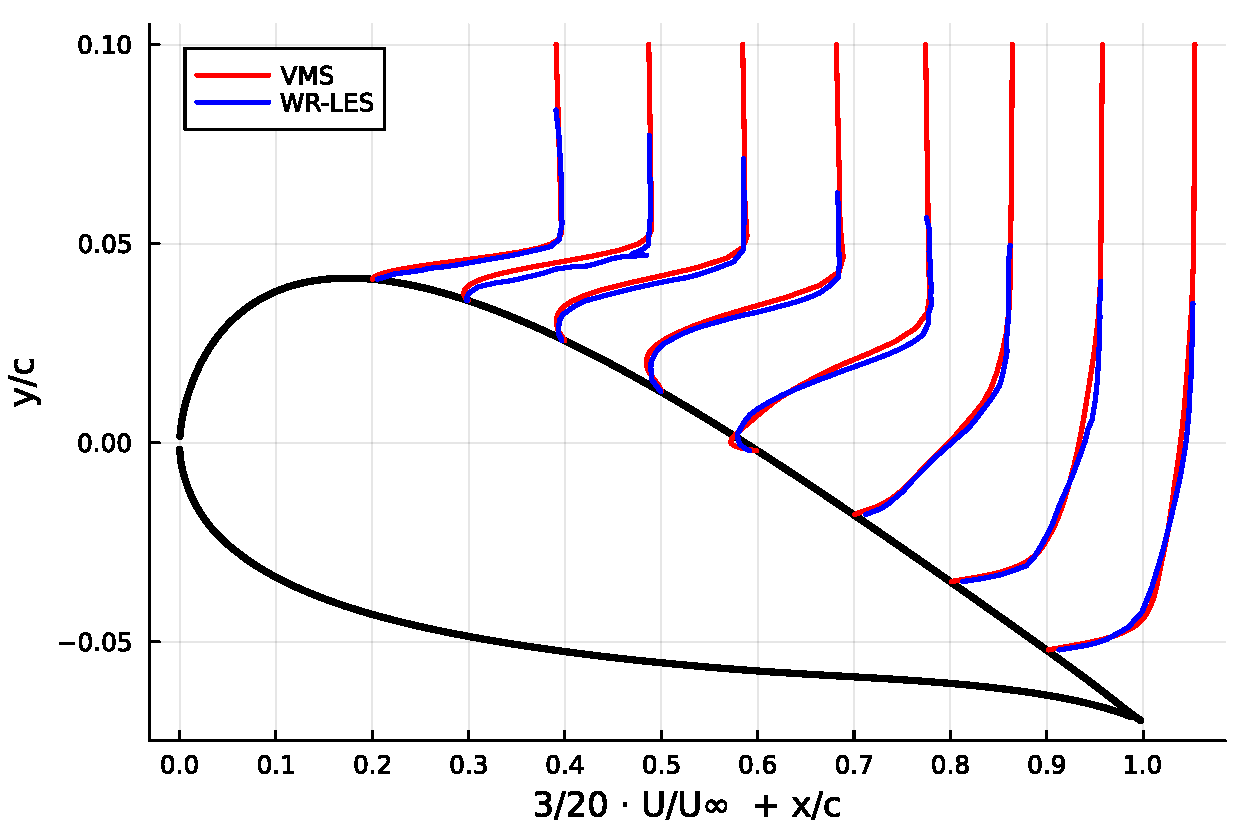
\includegraphics[width=0.6\textwidth]{sd7003s_hardcore.pdf}
                \caption{sd7003s and velocity profiles (re-scaled)}
            \end{figure} 
\end{frame}

\begin{frame}{Airfoil DU89 Reynolds 500000, AoA 1}
            \begin{figure}[h]
                \centering          
                    \centering
                    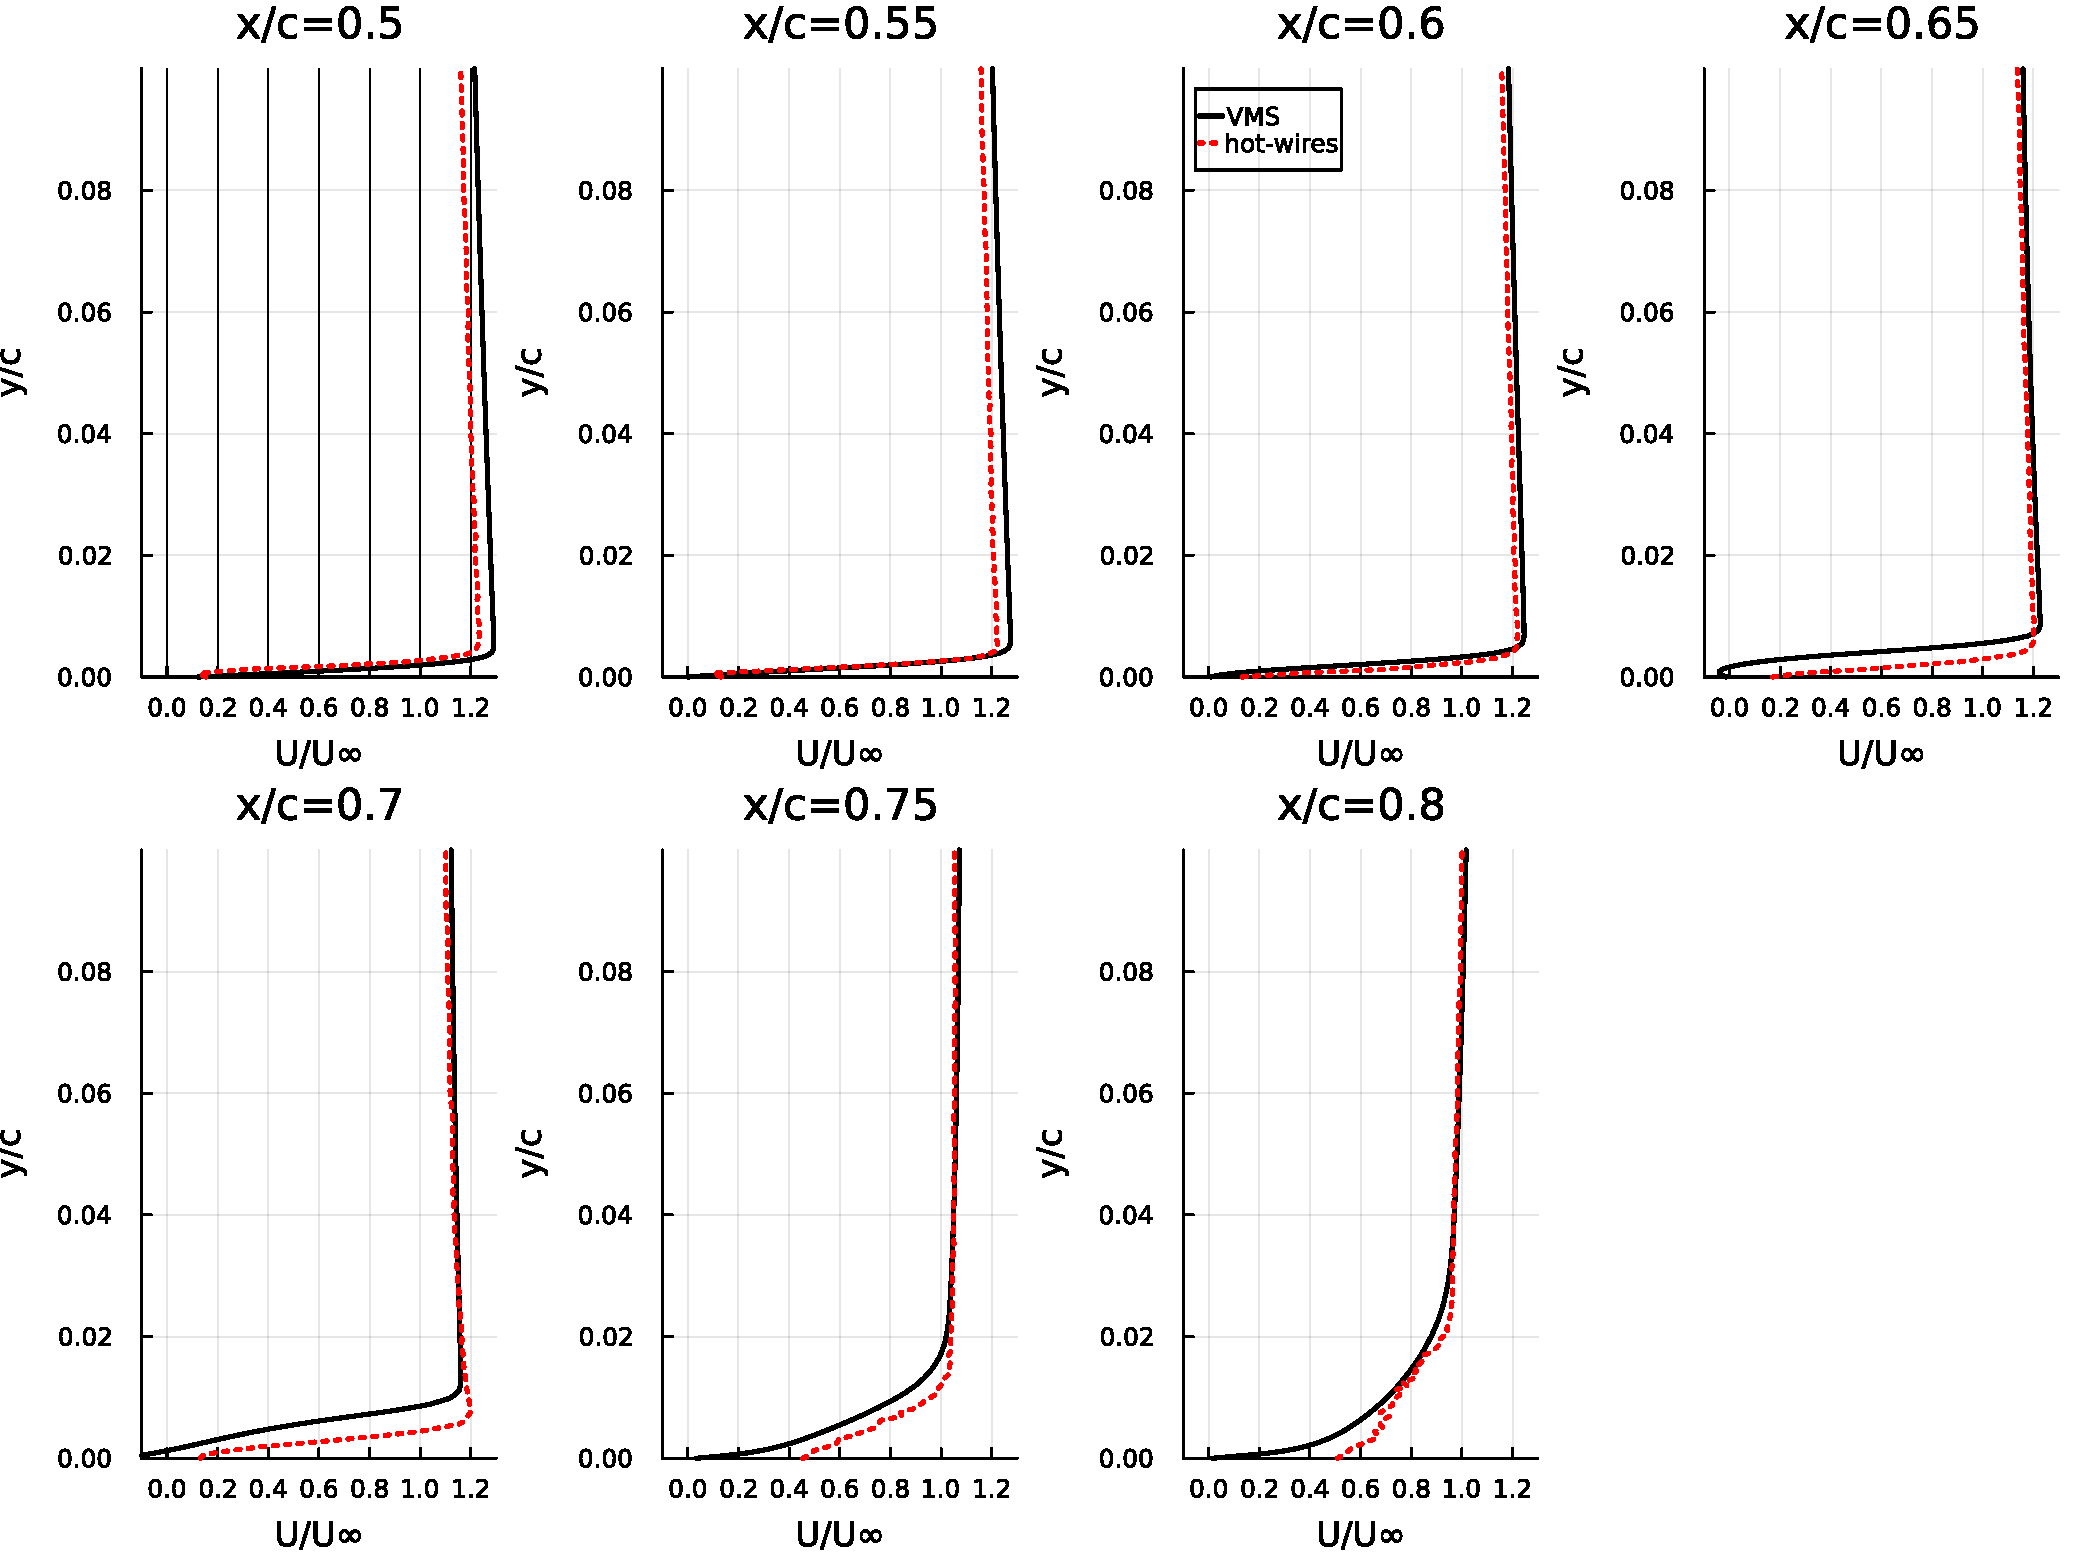
\includegraphics[width=0.6\textwidth]{Re500AoA1_VMSvsHW.pdf}
                    \caption{hot-wires and VMS velocity profiles}
                \end{figure} 
\end{frame}




\section{Adjoint method}
\begin{frame}{Adjoint Method}
    \begin{itemize}
        \item Airfoil optimization
        \item Require primal and adjoint simulation
        \item Complexity is independent of the number of parameters (eg control points on the airfoil)
    \end{itemize}

\end{frame}


\begin{frame}{NACA0012 $AoA=\ang{2.5}$, $Re=1000$ - drag minimization}
    \begin{figure}[h]
        \centering
        \begin{subfigure}[h]{0.45\textwidth}
            \centering
            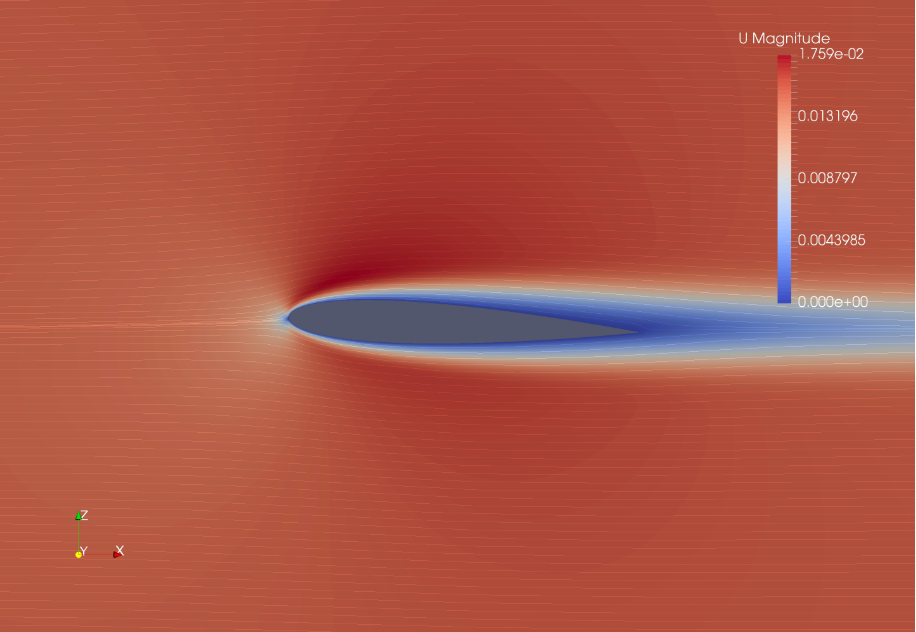
\includegraphics[width=\textwidth]{NACA0012_Uprimal.png}
        \end{subfigure}
        \hfill
        \begin{subfigure}[h]{0.45\textwidth}
            \centering
            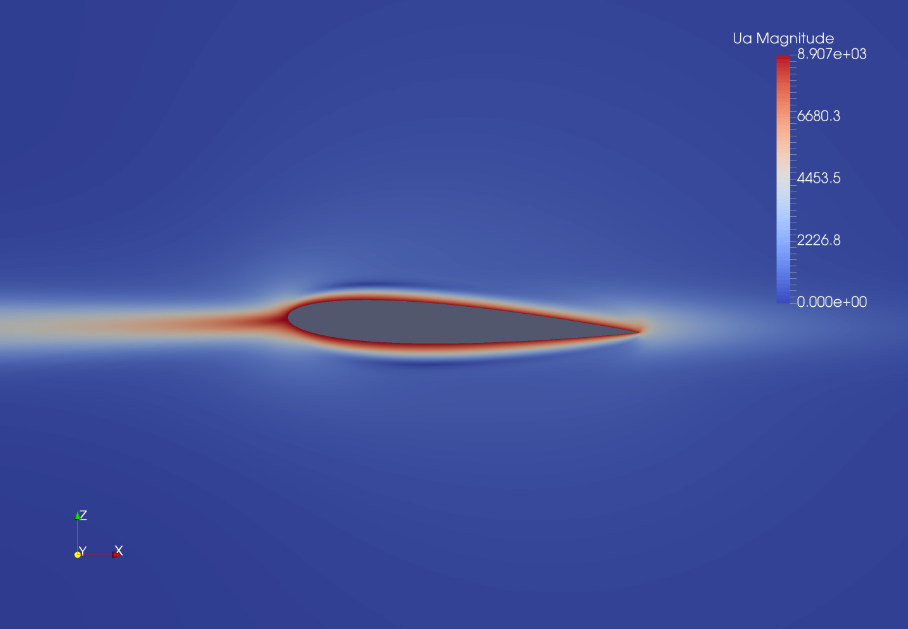
\includegraphics[width=\textwidth]{NACA0012_Uadjoint.png}
        \end{subfigure}
        \caption{Primal and Adjoint Velocity}
    \end{figure}
\end{frame}



\begin{frame}{NACA0012 $AoA=\ang{2.5}$, $Re=1000$ - drag minimization}
    \begin{figure}[h]
        \centering
        \begin{subfigure}[h]{0.45\textwidth}
            \centering
            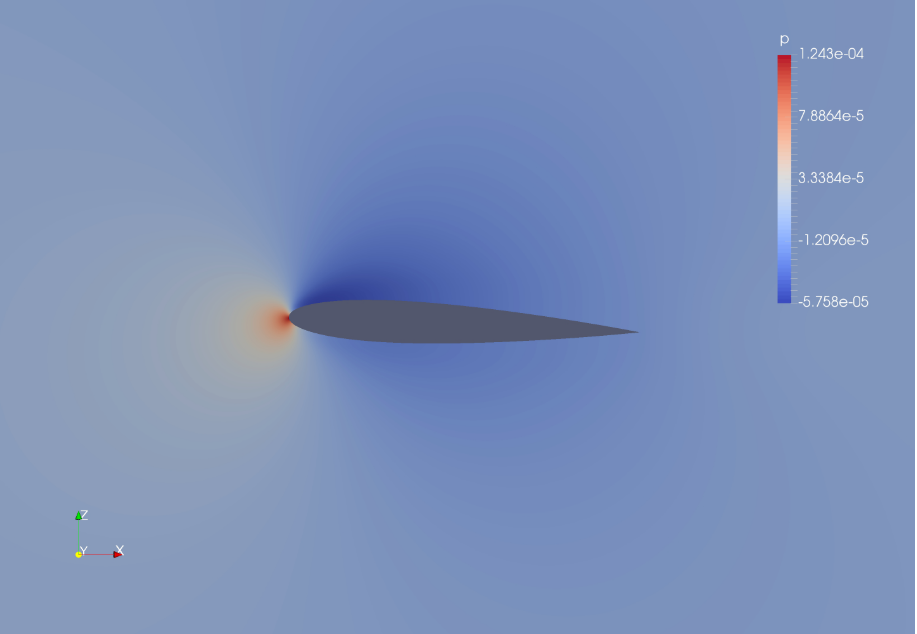
\includegraphics[width=\textwidth]{NACA0012_Pprimal.png}
        \end{subfigure}
        \hfill
        \begin{subfigure}[h]{0.45\textwidth}
            \centering
            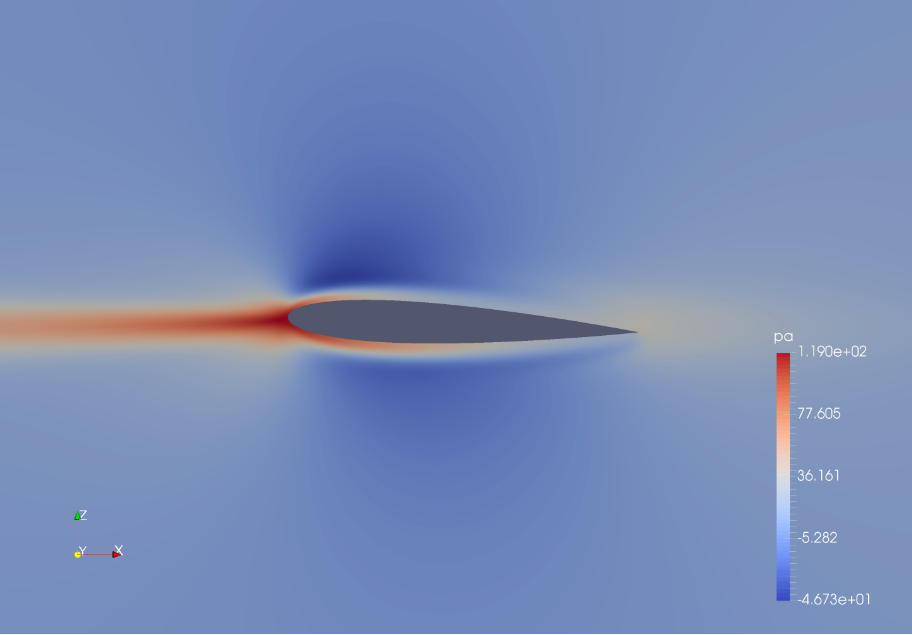
\includegraphics[width=\textwidth]{NACA0012_Padjoint.png}
        \end{subfigure}
        \caption{Primal and Adjoint pressure}
    \end{figure}
\end{frame}


\begin{frame}{NACA0012 $AoA=\ang{0.0}$, $Re=100$ - drag minimization}
    \begin{figure}[h]
        \centering
        \begin{subfigure}[h]{0.45\textwidth}
            \centering
            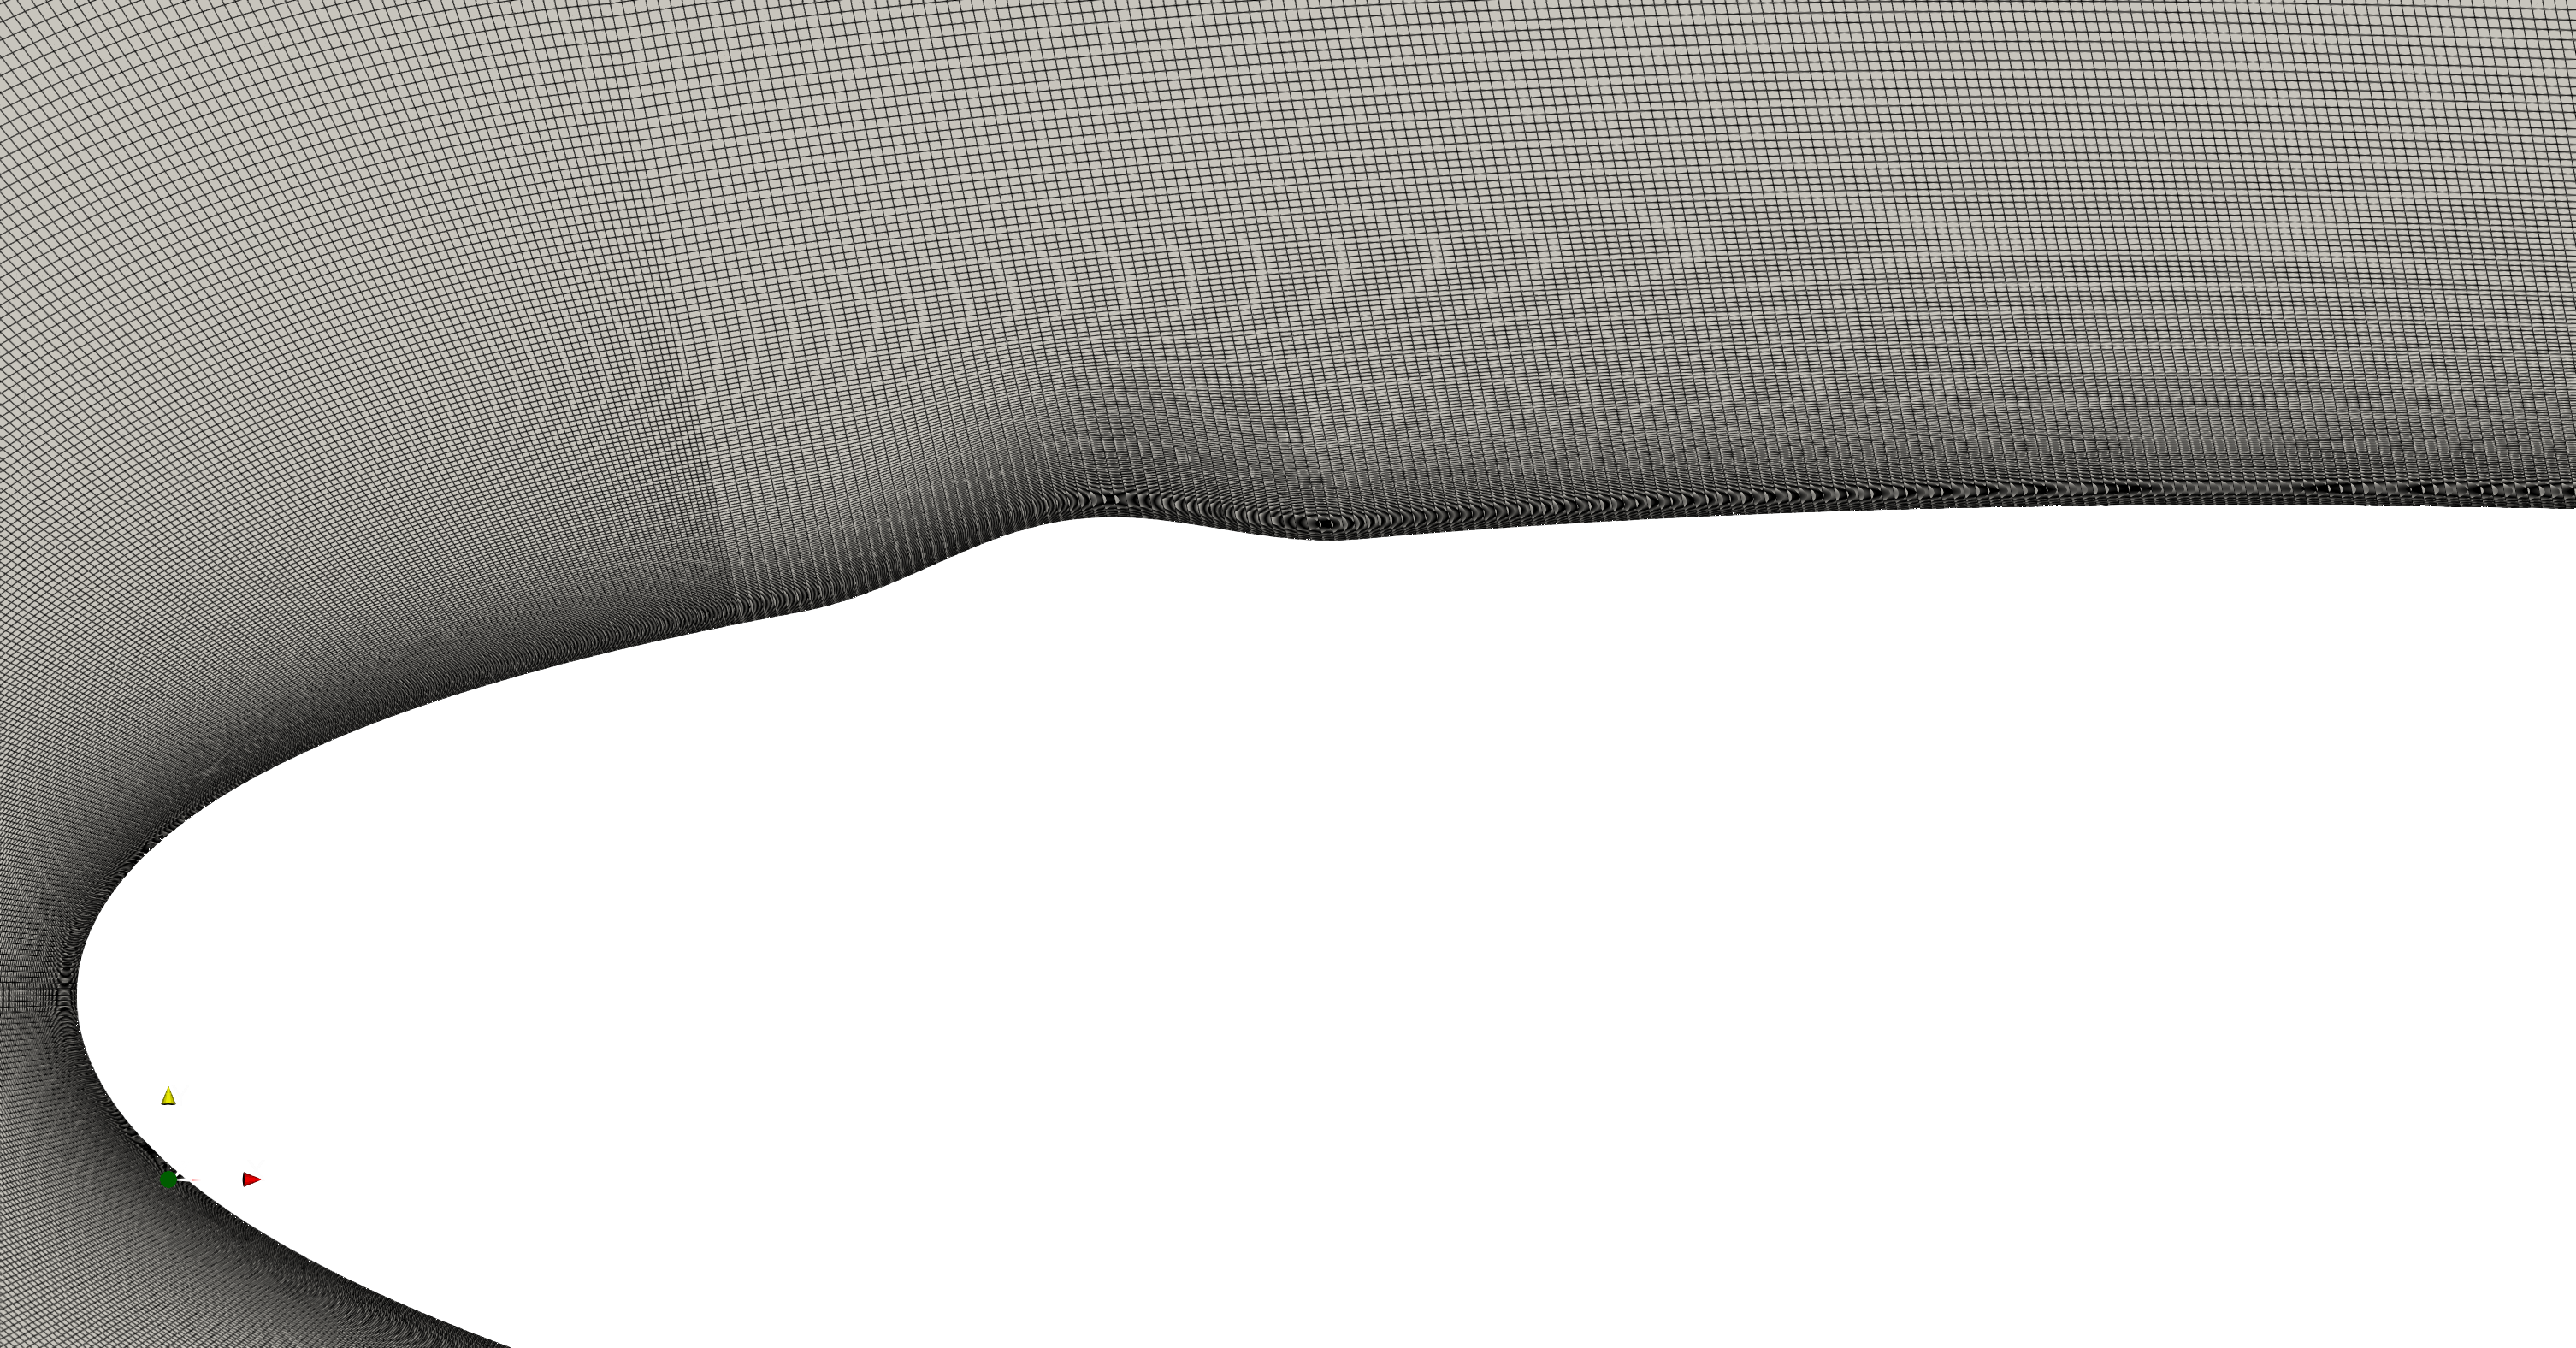
\includegraphics[width=\textwidth]{MeshDeformation.png}
            \caption{Local Mesh Deformation}
        \end{subfigure}
        \hfill
        \begin{subfigure}[h]{0.45\textwidth}
            \centering
            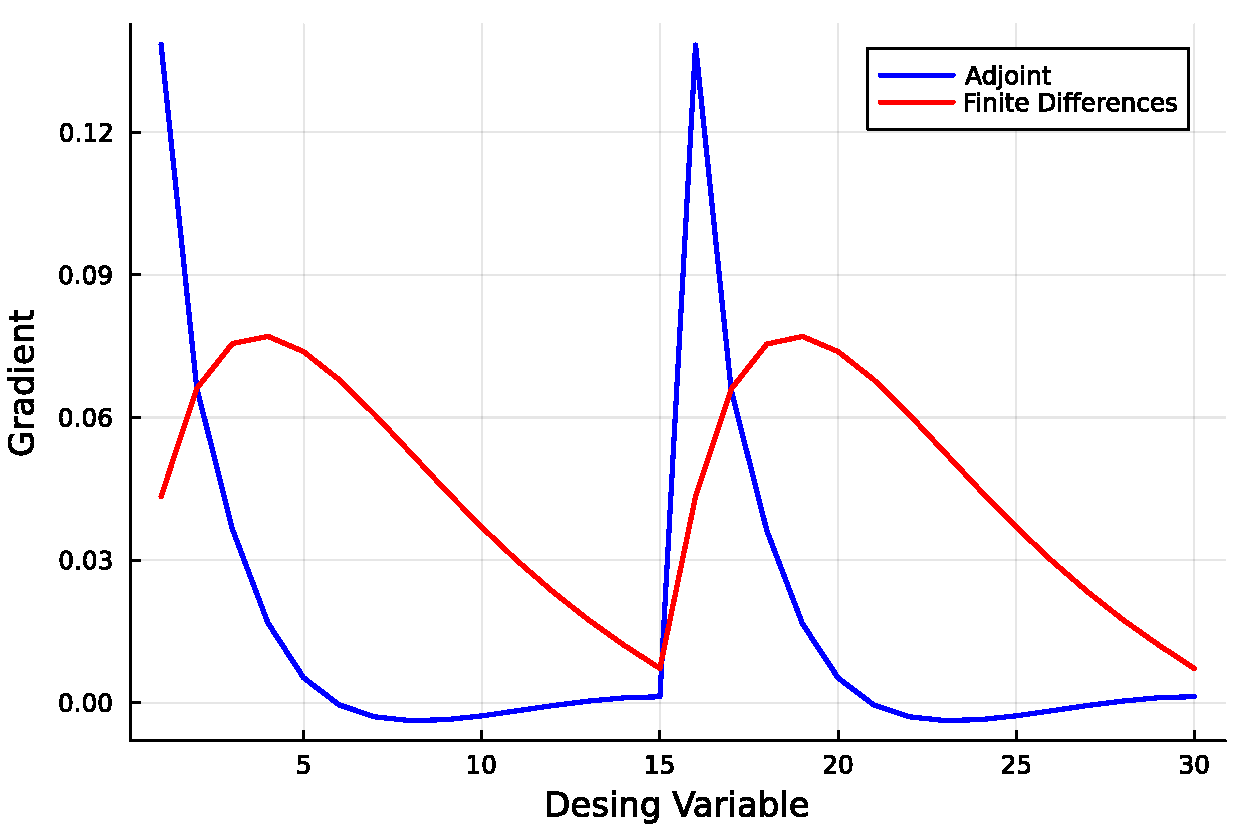
\includegraphics[width=\textwidth]{Adjoint_FD.pdf}
        \end{subfigure}
        \caption{Finite Difference and Adjoint gradient}
    \end{figure}
\end{frame}
\end{document}
